% Created by tikzDevice version 0.10.1 on 2018-02-17 17:12:17
% !TEX encoding = UTF-8 Unicode
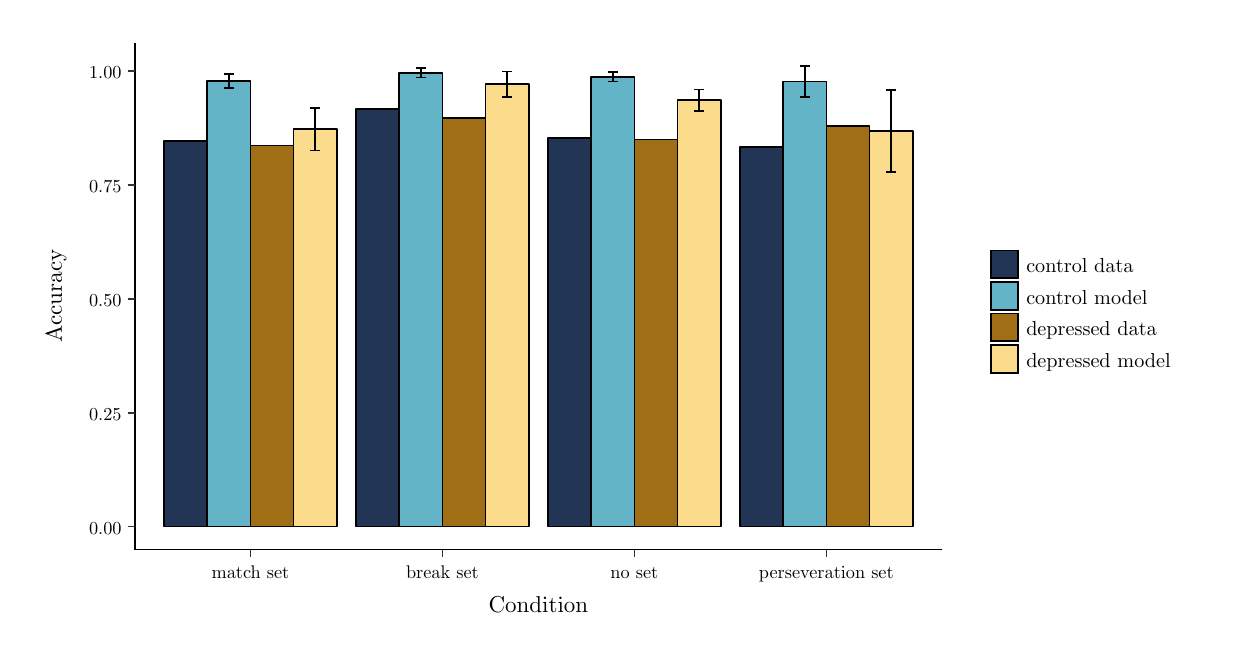
\begin{tikzpicture}[x=1pt,y=1pt]
\definecolor{fillColor}{RGB}{255,255,255}
\path[use as bounding box,fill=fillColor,fill opacity=0.00] (0,0) rectangle (433.62,216.81);
\begin{scope}
\path[clip] (  0.00,  0.00) rectangle (433.62,216.81);
\definecolor{drawColor}{RGB}{255,255,255}
\definecolor{fillColor}{RGB}{255,255,255}

\path[draw=drawColor,line width= 0.6pt,line join=round,line cap=round,fill=fillColor] (  0.00,  0.00) rectangle (433.62,216.81);
\end{scope}
\begin{scope}
\path[clip] ( 38.88, 28.22) rectangle (330.22,211.31);
\definecolor{fillColor}{RGB}{255,255,255}

\path[fill=fillColor] ( 38.88, 28.22) rectangle (330.22,211.31);
\definecolor{drawColor}{RGB}{0,0,0}
\definecolor{fillColor}{RGB}{250,220,140}

\path[draw=drawColor,line width= 0.6pt,line join=round,fill=fillColor] ( 96.11, 36.55) rectangle (111.72,180.14);
\definecolor{fillColor}{RGB}{160,110,20}

\path[draw=drawColor,line width= 0.6pt,line join=round,fill=fillColor] ( 80.50, 36.55) rectangle ( 96.11,174.19);
\definecolor{fillColor}{RGB}{100,180,200}

\path[draw=drawColor,line width= 0.6pt,line join=round,fill=fillColor] ( 64.90, 36.55) rectangle ( 80.50,197.58);
\definecolor{fillColor}{RGB}{35,53,85}

\path[draw=drawColor,line width= 0.6pt,line join=round,fill=fillColor] ( 49.29, 36.55) rectangle ( 64.90,175.84);
\definecolor{fillColor}{RGB}{250,220,140}

\path[draw=drawColor,line width= 0.6pt,line join=round,fill=fillColor] (165.48, 36.55) rectangle (181.08,196.44);
\definecolor{fillColor}{RGB}{160,110,20}

\path[draw=drawColor,line width= 0.6pt,line join=round,fill=fillColor] (149.87, 36.55) rectangle (165.48,184.06);
\definecolor{fillColor}{RGB}{100,180,200}

\path[draw=drawColor,line width= 0.6pt,line join=round,fill=fillColor] (134.26, 36.55) rectangle (149.87,200.49);
\definecolor{fillColor}{RGB}{35,53,85}

\path[draw=drawColor,line width= 0.6pt,line join=round,fill=fillColor] (118.65, 36.55) rectangle (134.26,187.35);
\definecolor{fillColor}{RGB}{250,220,140}

\path[draw=drawColor,line width= 0.6pt,line join=round,fill=fillColor] (234.84, 36.55) rectangle (250.45,190.59);
\definecolor{fillColor}{RGB}{160,110,20}

\path[draw=drawColor,line width= 0.6pt,line join=round,fill=fillColor] (219.23, 36.55) rectangle (234.84,176.39);
\definecolor{fillColor}{RGB}{100,180,200}

\path[draw=drawColor,line width= 0.6pt,line join=round,fill=fillColor] (203.63, 36.55) rectangle (219.23,199.07);
\definecolor{fillColor}{RGB}{35,53,85}

\path[draw=drawColor,line width= 0.6pt,line join=round,fill=fillColor] (188.02, 36.55) rectangle (203.63,176.93);
\definecolor{fillColor}{RGB}{250,220,140}

\path[draw=drawColor,line width= 0.6pt,line join=round,fill=fillColor] (304.20, 36.55) rectangle (319.81,179.38);
\definecolor{fillColor}{RGB}{160,110,20}

\path[draw=drawColor,line width= 0.6pt,line join=round,fill=fillColor] (288.60, 36.55) rectangle (304.20,181.32);
\definecolor{fillColor}{RGB}{100,180,200}

\path[draw=drawColor,line width= 0.6pt,line join=round,fill=fillColor] (272.99, 36.55) rectangle (288.60,197.38);
\definecolor{fillColor}{RGB}{35,53,85}

\path[draw=drawColor,line width= 0.6pt,line join=round,fill=fillColor] (257.38, 36.55) rectangle (272.99,173.64);

\path[draw=drawColor,line width= 0.6pt,line join=round] (102.18,187.89) --
	(105.65,187.89);

\path[draw=drawColor,line width= 0.6pt,line join=round] (103.91,187.89) --
	(103.91,172.38);

\path[draw=drawColor,line width= 0.6pt,line join=round] (102.18,172.38) --
	(105.65,172.38);

\path[draw=drawColor,line width= 0.6pt,line join=round] ( 70.97,200.06) --
	( 74.43,200.06);

\path[draw=drawColor,line width= 0.6pt,line join=round] ( 72.70,200.06) --
	( 72.70,195.09);

\path[draw=drawColor,line width= 0.6pt,line join=round] ( 70.97,195.09) --
	( 74.43,195.09);

\path[draw=drawColor,line width= 0.6pt,line join=round] (171.54,201.03) --
	(175.01,201.03);

\path[draw=drawColor,line width= 0.6pt,line join=round] (173.28,201.03) --
	(173.28,191.86);

\path[draw=drawColor,line width= 0.6pt,line join=round] (171.54,191.86) --
	(175.01,191.86);

\path[draw=drawColor,line width= 0.6pt,line join=round] (140.33,202.17) --
	(143.80,202.17);

\path[draw=drawColor,line width= 0.6pt,line join=round] (142.06,202.17) --
	(142.06,198.81);

\path[draw=drawColor,line width= 0.6pt,line join=round] (140.33,198.81) --
	(143.80,198.81);

\path[draw=drawColor,line width= 0.6pt,line join=round] (240.91,194.44) --
	(244.38,194.44);

\path[draw=drawColor,line width= 0.6pt,line join=round] (242.64,194.44) --
	(242.64,186.75);

\path[draw=drawColor,line width= 0.6pt,line join=round] (240.91,186.75) --
	(244.38,186.75);

\path[draw=drawColor,line width= 0.6pt,line join=round] (209.70,200.79) --
	(213.16,200.79);

\path[draw=drawColor,line width= 0.6pt,line join=round] (211.43,200.79) --
	(211.43,197.36);

\path[draw=drawColor,line width= 0.6pt,line join=round] (209.70,197.36) --
	(213.16,197.36);

\path[draw=drawColor,line width= 0.6pt,line join=round] (310.27,194.17) --
	(313.74,194.17);

\path[draw=drawColor,line width= 0.6pt,line join=round] (312.01,194.17) --
	(312.01,164.58);

\path[draw=drawColor,line width= 0.6pt,line join=round] (310.27,164.58) --
	(313.74,164.58);

\path[draw=drawColor,line width= 0.6pt,line join=round] (279.06,202.99) --
	(282.53,202.99);

\path[draw=drawColor,line width= 0.6pt,line join=round] (280.79,202.99) --
	(280.79,191.77);

\path[draw=drawColor,line width= 0.6pt,line join=round] (279.06,191.77) --
	(282.53,191.77);
\end{scope}
\begin{scope}
\path[clip] (  0.00,  0.00) rectangle (433.62,216.81);
\definecolor{drawColor}{RGB}{0,0,0}

\path[draw=drawColor,line width= 0.6pt,line join=round] ( 38.88, 28.22) --
	( 38.88,211.31);
\end{scope}
\begin{scope}
\path[clip] (  0.00,  0.00) rectangle (433.62,216.81);
\definecolor{drawColor}{RGB}{0,0,0}

\node[text=drawColor,anchor=base east,inner sep=0pt, outer sep=0pt, scale=  0.66] at ( 33.93, 33.82) {0.00};

\node[text=drawColor,anchor=base east,inner sep=0pt, outer sep=0pt, scale=  0.66] at ( 33.93, 74.95) {0.25};

\node[text=drawColor,anchor=base east,inner sep=0pt, outer sep=0pt, scale=  0.66] at ( 33.93,116.08) {0.50};

\node[text=drawColor,anchor=base east,inner sep=0pt, outer sep=0pt, scale=  0.66] at ( 33.93,157.21) {0.75};

\node[text=drawColor,anchor=base east,inner sep=0pt, outer sep=0pt, scale=  0.66] at ( 33.93,198.34) {1.00};
\end{scope}
\begin{scope}
\path[clip] (  0.00,  0.00) rectangle (433.62,216.81);
\definecolor{drawColor}{gray}{0.20}

\path[draw=drawColor,line width= 0.6pt,line join=round] ( 36.13, 36.55) --
	( 38.88, 36.55);

\path[draw=drawColor,line width= 0.6pt,line join=round] ( 36.13, 77.67) --
	( 38.88, 77.67);

\path[draw=drawColor,line width= 0.6pt,line join=round] ( 36.13,118.80) --
	( 38.88,118.80);

\path[draw=drawColor,line width= 0.6pt,line join=round] ( 36.13,159.93) --
	( 38.88,159.93);

\path[draw=drawColor,line width= 0.6pt,line join=round] ( 36.13,201.06) --
	( 38.88,201.06);
\end{scope}
\begin{scope}
\path[clip] (  0.00,  0.00) rectangle (433.62,216.81);
\definecolor{drawColor}{RGB}{0,0,0}

\path[draw=drawColor,line width= 0.6pt,line join=round] ( 38.88, 28.22) --
	(330.22, 28.22);
\end{scope}
\begin{scope}
\path[clip] (  0.00,  0.00) rectangle (433.62,216.81);
\definecolor{drawColor}{gray}{0.20}

\path[draw=drawColor,line width= 0.6pt,line join=round] ( 80.50, 25.47) --
	( 80.50, 28.22);

\path[draw=drawColor,line width= 0.6pt,line join=round] (149.87, 25.47) --
	(149.87, 28.22);

\path[draw=drawColor,line width= 0.6pt,line join=round] (219.23, 25.47) --
	(219.23, 28.22);

\path[draw=drawColor,line width= 0.6pt,line join=round] (288.60, 25.47) --
	(288.60, 28.22);
\end{scope}
\begin{scope}
\path[clip] (  0.00,  0.00) rectangle (433.62,216.81);
\definecolor{drawColor}{RGB}{0,0,0}

\node[text=drawColor,anchor=base,inner sep=0pt, outer sep=0pt, scale=  0.66] at ( 80.50, 17.82) {match set};

\node[text=drawColor,anchor=base,inner sep=0pt, outer sep=0pt, scale=  0.66] at (149.87, 17.82) {break set};

\node[text=drawColor,anchor=base,inner sep=0pt, outer sep=0pt, scale=  0.66] at (219.23, 17.82) {no set};

\node[text=drawColor,anchor=base,inner sep=0pt, outer sep=0pt, scale=  0.66] at (288.60, 17.82) {perseveration set};
\end{scope}
\begin{scope}
\path[clip] (  0.00,  0.00) rectangle (433.62,216.81);
\definecolor{drawColor}{RGB}{0,0,0}

\node[text=drawColor,anchor=base,inner sep=0pt, outer sep=0pt, scale=  0.83] at (184.55,  5.50) {Condition};
\end{scope}
\begin{scope}
\path[clip] (  0.00,  0.00) rectangle (433.62,216.81);
\definecolor{drawColor}{RGB}{0,0,0}

\node[text=drawColor,rotate= 90.00,anchor=base,inner sep=0pt, outer sep=0pt, scale=  0.83] at ( 12.32,119.77) {Accuracy};
\end{scope}
\begin{scope}
\path[clip] (  0.00,  0.00) rectangle (433.62,216.81);
\definecolor{fillColor}{RGB}{255,255,255}

\path[fill=fillColor] (341.60, 85.74) rectangle (428.12,153.80);
\end{scope}
\begin{scope}
\path[clip] (  0.00,  0.00) rectangle (433.62,216.81);
\definecolor{drawColor}{RGB}{0,0,0}
\definecolor{fillColor}{RGB}{35,53,85}

\path[draw=drawColor,line width= 0.6pt,line cap=round,fill=fillColor] (348.00,126.28) rectangle (357.96,136.24);
\end{scope}
\begin{scope}
\path[clip] (  0.00,  0.00) rectangle (433.62,216.81);
\definecolor{drawColor}{RGB}{0,0,0}
\definecolor{fillColor}{RGB}{100,180,200}

\path[draw=drawColor,line width= 0.6pt,line cap=round,fill=fillColor] (348.00,114.90) rectangle (357.96,124.86);
\end{scope}
\begin{scope}
\path[clip] (  0.00,  0.00) rectangle (433.62,216.81);
\definecolor{drawColor}{RGB}{0,0,0}
\definecolor{fillColor}{RGB}{160,110,20}

\path[draw=drawColor,line width= 0.6pt,line cap=round,fill=fillColor] (348.00,103.52) rectangle (357.96,113.48);
\end{scope}
\begin{scope}
\path[clip] (  0.00,  0.00) rectangle (433.62,216.81);
\definecolor{drawColor}{RGB}{0,0,0}
\definecolor{fillColor}{RGB}{250,220,140}

\path[draw=drawColor,line width= 0.6pt,line cap=round,fill=fillColor] (348.00, 92.14) rectangle (357.96,102.10);
\end{scope}
\begin{scope}
\path[clip] (  0.00,  0.00) rectangle (433.62,216.81);
\definecolor{drawColor}{RGB}{0,0,0}

\node[text=drawColor,anchor=base west,inner sep=0pt, outer sep=0pt, scale=  0.73] at (360.84,128.23) {control data};
\end{scope}
\begin{scope}
\path[clip] (  0.00,  0.00) rectangle (433.62,216.81);
\definecolor{drawColor}{RGB}{0,0,0}

\node[text=drawColor,anchor=base west,inner sep=0pt, outer sep=0pt, scale=  0.73] at (360.84,116.85) {control model};
\end{scope}
\begin{scope}
\path[clip] (  0.00,  0.00) rectangle (433.62,216.81);
\definecolor{drawColor}{RGB}{0,0,0}

\node[text=drawColor,anchor=base west,inner sep=0pt, outer sep=0pt, scale=  0.73] at (360.84,105.47) {depressed data};
\end{scope}
\begin{scope}
\path[clip] (  0.00,  0.00) rectangle (433.62,216.81);
\definecolor{drawColor}{RGB}{0,0,0}

\node[text=drawColor,anchor=base west,inner sep=0pt, outer sep=0pt, scale=  0.73] at (360.84, 94.09) {depressed model};
\end{scope}
\end{tikzpicture}
